\documentclass{article}

\usepackage[russian]{babel}    %enable russian languge
\usepackage[utf8]{inputenc}
\usepackage[T2A]{fontenc}

\usepackage[a4paper, includefoot, 
            left=1.0cm, right=1.0cm, 
            top=1.5cm, bottom=1.5cm, 
            headsep=1cm, footskip=1cm]{geometry}
\usepackage{amsmath}
\usepackage{amssymb}
\usepackage{array}
\usepackage{caption}
\usepackage{longtable}
\usepackage{multirow}

%\renewcommand{\rmdefault}{ftm}
%\usepackage{concrete}

\pagestyle{plain}

\usepackage{graphicx}
\graphicspath{{pics/}}

\usepackage[fontsize=12]{scrextend}
\renewcommand{\baselinestretch}{1.5}

\setcounter{table}{1}

%%%%%%%%%%%%%%%%%%%%%%%%%%%%%%%%%%%%%%%%%%%%%%%%%%%%%%%%%%%%%%%%%%%
%                        My commands                              %
%%%%%%%%%%%%%%%%%%%%%%%%%%%%%%%%%%%%%%%%%%%%%%%%%%%%%%%%%%%%%%%%%%%
\newcommand{\n}{\vspace{\baselineskip}}
\newcommand{\ntb}{\tabularnewline}
\newcommand{\tabscale}[1]{\renewcommand{\arraystretch}{#1}}


\newcommand{\tabcapt}[1]{{\center{Таб. \thetable:  #1}\addtocounter{table}{1}\\ \quad \\}}
\newcommand{\piccapt}[1]{\addtocounter{figure}{1}{\center{Рис. \thefigure: #1}\\ \quad \\}}

% \pich{scale}{pic}{caption}
\newcommand{\pic}[3]	
{
\noindent
\begin{minipage}{\linewidth}
  \center{\includegraphics[width = #1\linewidth]{#2}}
  \piccapt{#3}
\end{minipage}
}

% \pich{scale}{minipage height}{pic}{caption}
\newcommand{\pich}[4]
{
\noindent
\begin{minipage}{\linewidth}
  \center{\includegraphics[width = #1\linewidth, height = #2]{#3}}
  \captionof{figure}{#4}
\end{minipage}
}
%%%%%%%%%%%%%%%%%%%%%%%%%%%%%%%%%%%%%%%%%%%%%%%%%%%%%%%%%%%%%%%%%%%%


\begin{document}

\begin{center}{
\normalsize Санкт-Петербургский Государственный Политехнический университет\\
Институт Прикладной Математики и Механики\\
[7cm]
} 
\Huge Отчет\\ 
\large по вычислительной лабораторной работе:\\
\large	
\textbf{"Стационарное ламинарное обтекание круглого цилиндра"} \\
[5cm]
\begin{flushleft}
\quad\quad Выполнил:  \hspace{10 cm} \parbox[t]{4.5cm}{Пинаев И. А. \\ студент гр.33601/1 }\\
\end{flushleft}
\vfill
{\large Санкт-Петербург \\ 2014} 
\end{center}
\thispagestyle{empty}

\newpage

\section{Задание}
\noindent Выполнить расчет стационарного ламинарного обтекания круглого цилиндра потоком  вязкой  несжимаемой  жидкости  в  предположении о симметрии течения относительно срединного сечения цилиндра. 

\section{Постановка задачи}
	
\pic{0.7}{problem}{Расчетная область.}
\pic{0.7}{problem_grid}{Расчетная сетка.}

\noindent На рисунке 1 представлена расчетная область $ABEF$, построенная для расчета внешнего обтекания  круглого  цилиндра $IH$ диаметром $d$ в предположении о симметрии течения относительно линии $AF$. Границы $AB$ и $EF$ прямоугольной расчетной области отнесены на 10 калибров вверх и вниз по потоку от лобовой ($I$) и кормовой ($H$) точек цилиндра. Также на 10 калибров от цилиндра отстоит верхняя граница $ВЕ$. Расчетная область состоит из четырех блоков (см. рис. 1 и 2): $ABCJ$, $CDMK$, $DEFG$, $IJGH$. Вспомогательный блок $IJGH$ (блок 4) вводится с целью обеспечения малой скошенности ячеек расчетной сетки в окрестности твердой стенки. В конфигурации расчетной области, представленной на рисунках 1 и 2, точки, задающие геометрию блока $IJGH$, имеют следующие координаты: $J - x = -d$, $y = 0$, $K - x = -0.75d$, $y = 0.75d$; $L - x = 0$, $y = 1d$;  $M - x = 0.75d$,  $y = 0.75d$; $G - x = d$, $y = 0$. 

\n
\noindent Расчетная сетка (рис. 2) построена в соответствии с данными, приведенными в таблице ниже: 
\begin{center}
  \begin{tabular}{p{5.2cm}||c|c|c|c|c|c}
  Сегмент               & $AB, EF$ & $KC, MD$ & $AJ, BC, GF, DF$ & $JI, HG$ & $KM, CD$ & $JK, MG$ \\
  \hline 	
  Число узлов           & $39$  & 31 & 61 & 11 & 17 & 9   \\
  \hline 	
  Коэффициент сгущения  & $1.06$ & 1.07 & 1.02 или 0.98 & 1.1 & 1.0 & 1.0 \\
  \end{tabular}
\end{center}

\newpage
\section{Анализ результатов}

\subsection{Распределение вектора скорости}

\begin{minipage}{\linewidth}
  \begin{minipage}{0.49\linewidth}
    \center{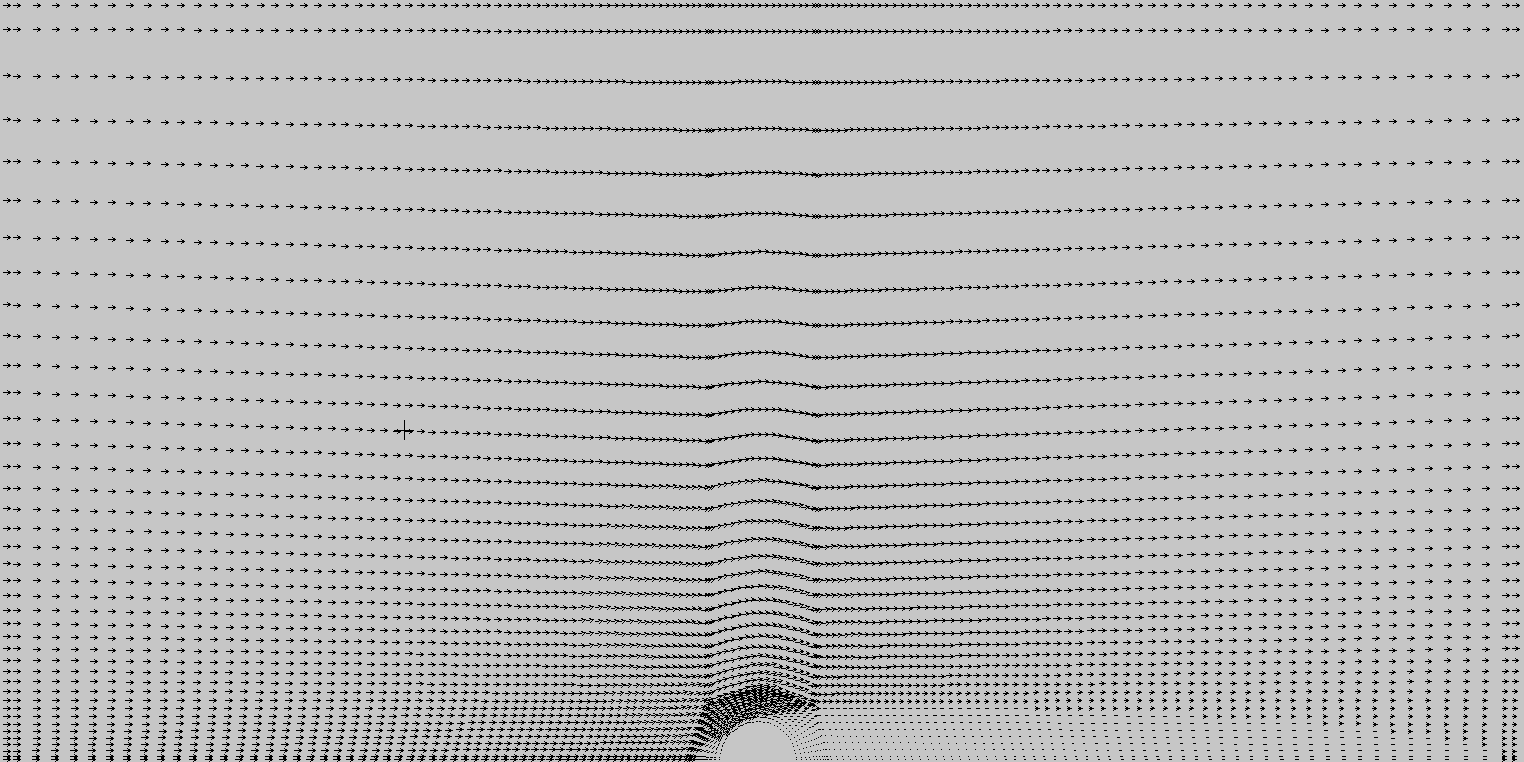
\includegraphics[width = \linewidth]{re40_vec} \\ (a)}
  \end{minipage}
  \hfill
  \begin{minipage}{0.49\linewidth}
    \center{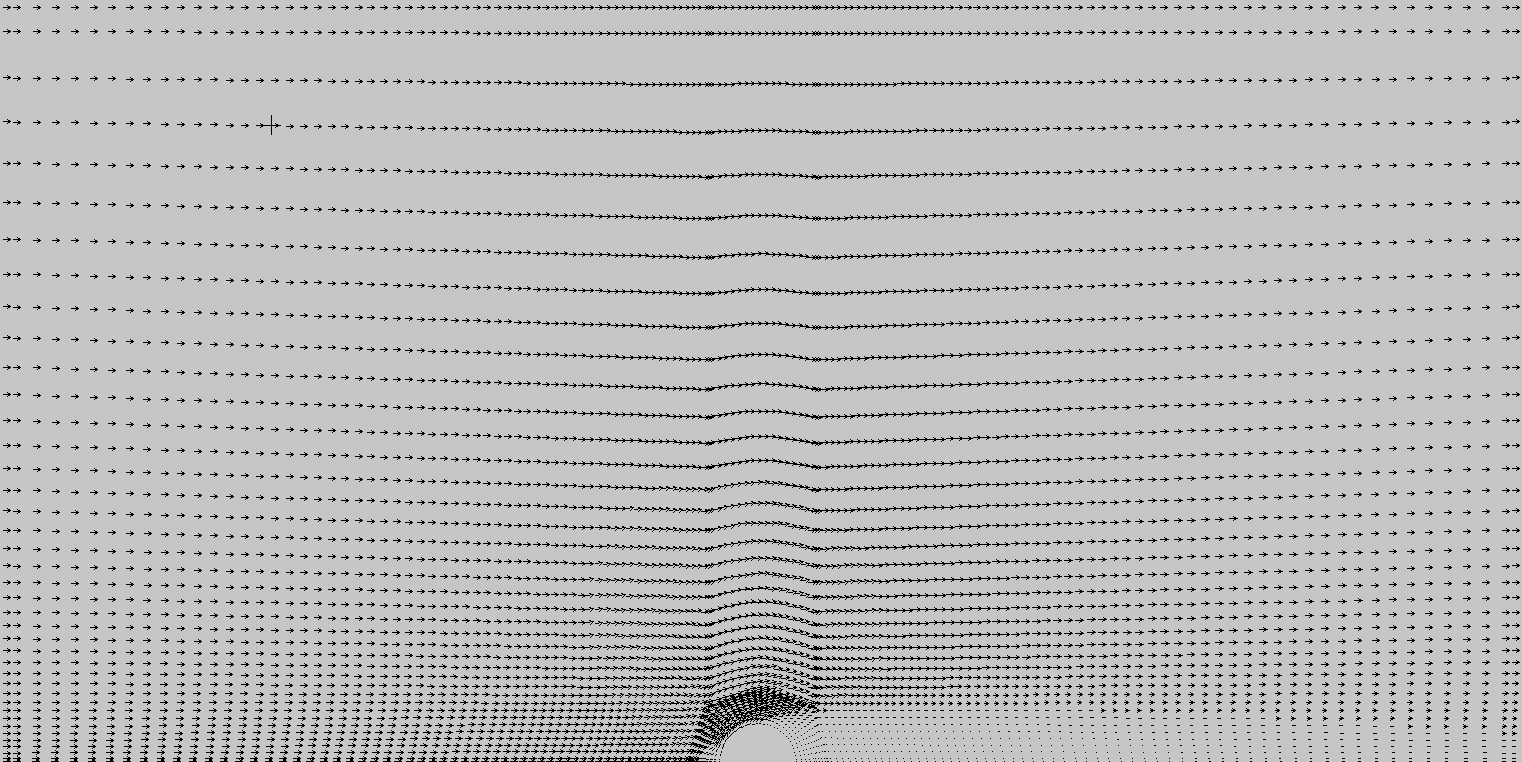
\includegraphics[width = \linewidth]{re80_vel_vec} \\ (б)}
  \end{minipage}
\end{minipage}

\vspace{2mm}
\noindent
\begin{minipage}{\linewidth}
  \begin{minipage}{0.49\linewidth}
    \center{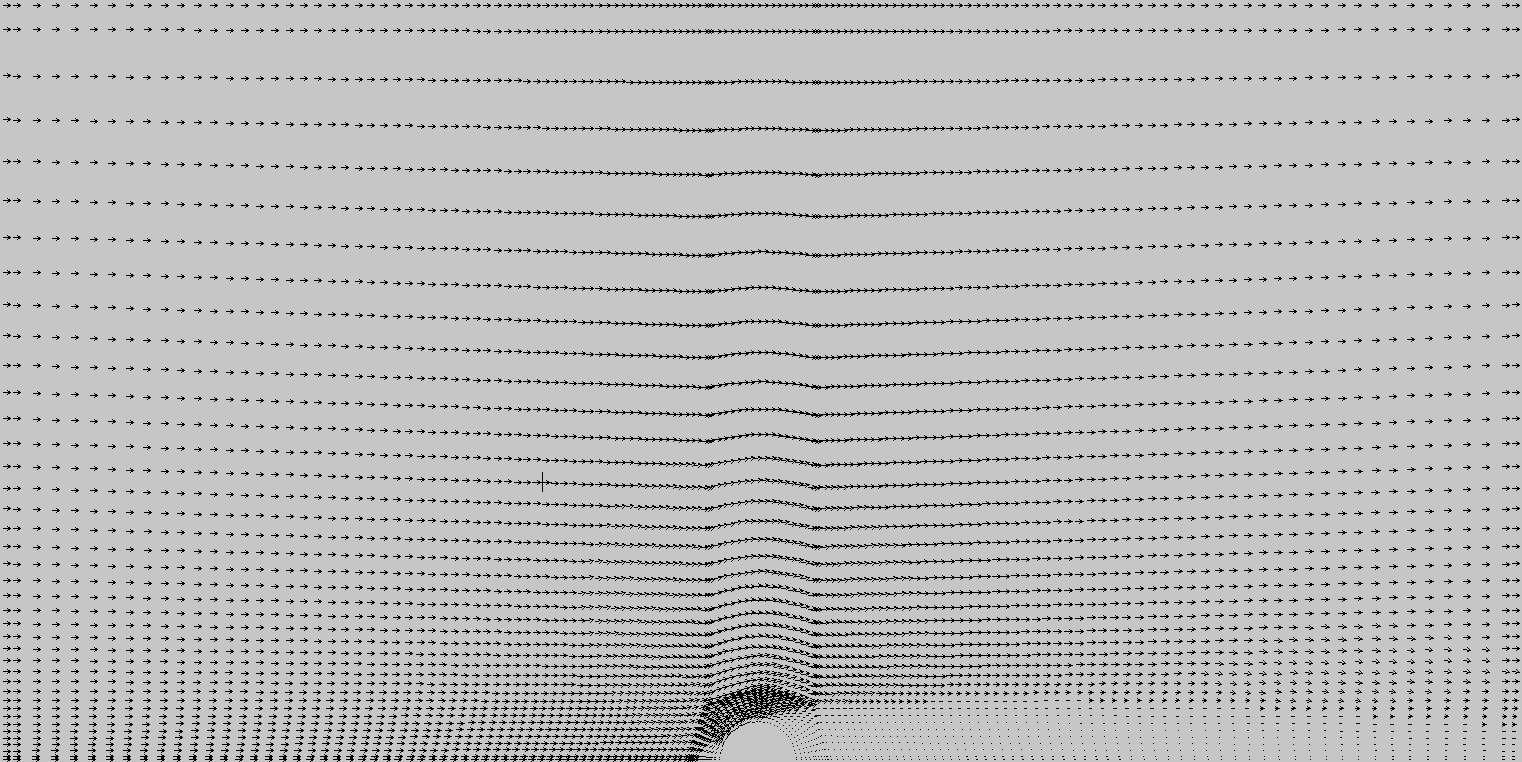
\includegraphics[width = \linewidth]{re130_vel_vec} \\ (в)}
  \end{minipage}
  \hfill
  \begin{minipage}{0.49\linewidth}
    \center{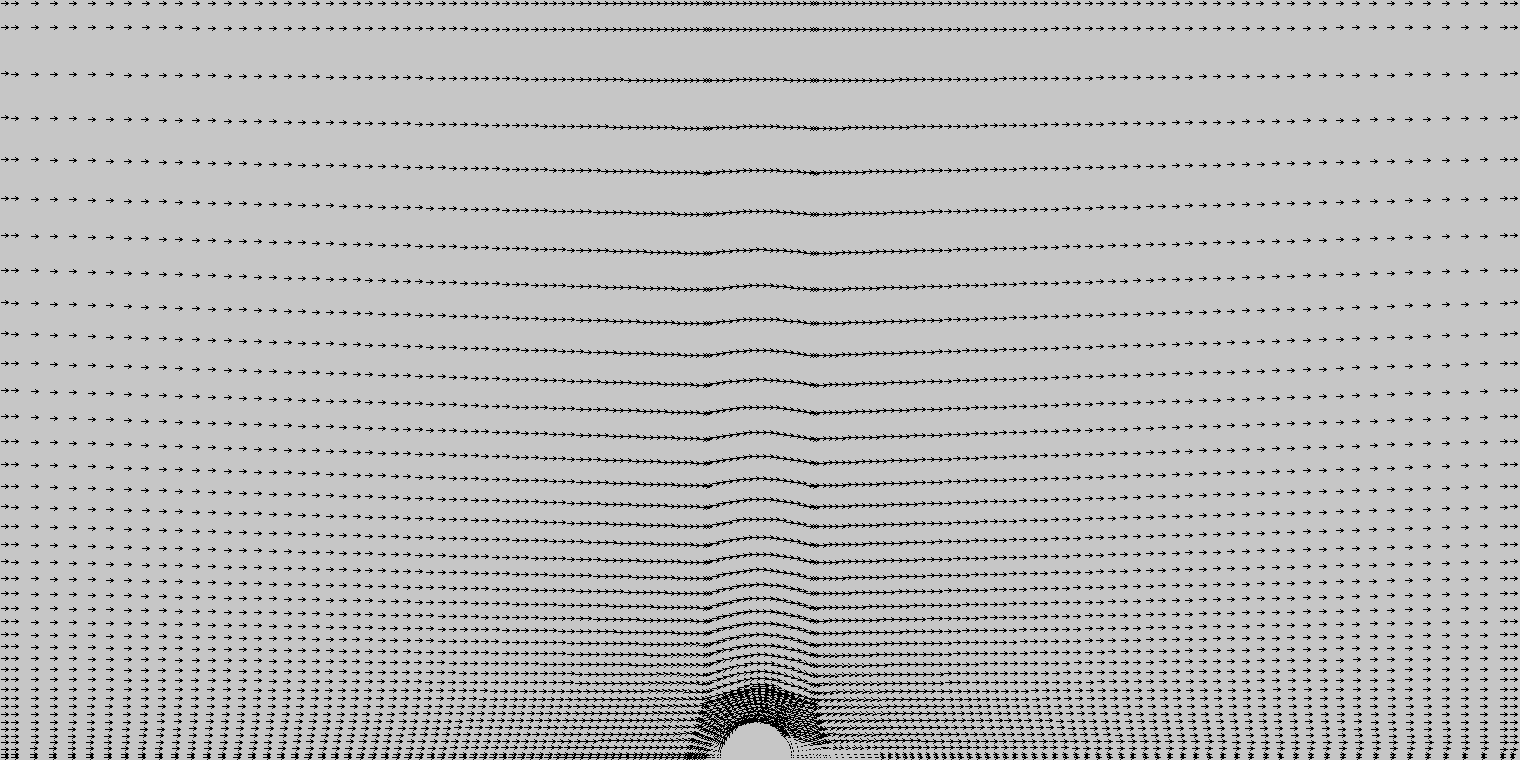
\includegraphics[width = \linewidth]{vel_vec} \\ (г)}
  \end{minipage}
\end{minipage}
\piccapt{Распределение вектора скорости: (a) - $Re = 40$, (б) - $Re = 80$, \\(в) - $Re = 130$, (г) - невязкая жидкость.}

\noindent На рисунке 3 можно видеть, что с увеличением числа Рейнольдса $Re$	 увеличивается длина рециркуляционной зоны, в то время как в потоке невязкой жидкости (рис 3(г)) рециркуляционная зона практически отсутствует.

\newpage
\subsection{Распределение продольной компоненты скорости}

\begin{minipage}{\linewidth}
  \begin{minipage}{0.49\linewidth}
    \center{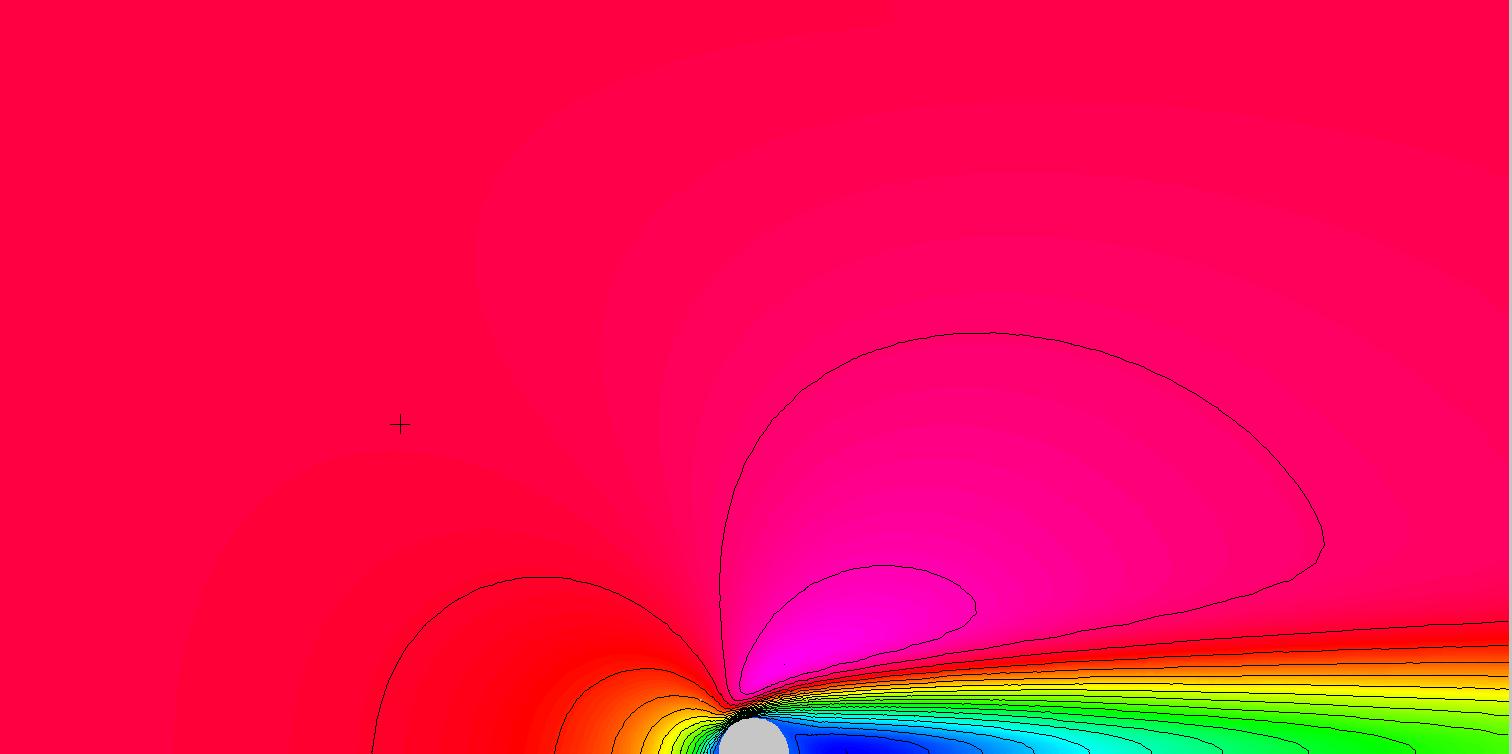
\includegraphics[width = \linewidth]{re40_vel_x} \\ (a)}
  \end{minipage}
  \hfill
  \begin{minipage}{0.49\linewidth}
    \center{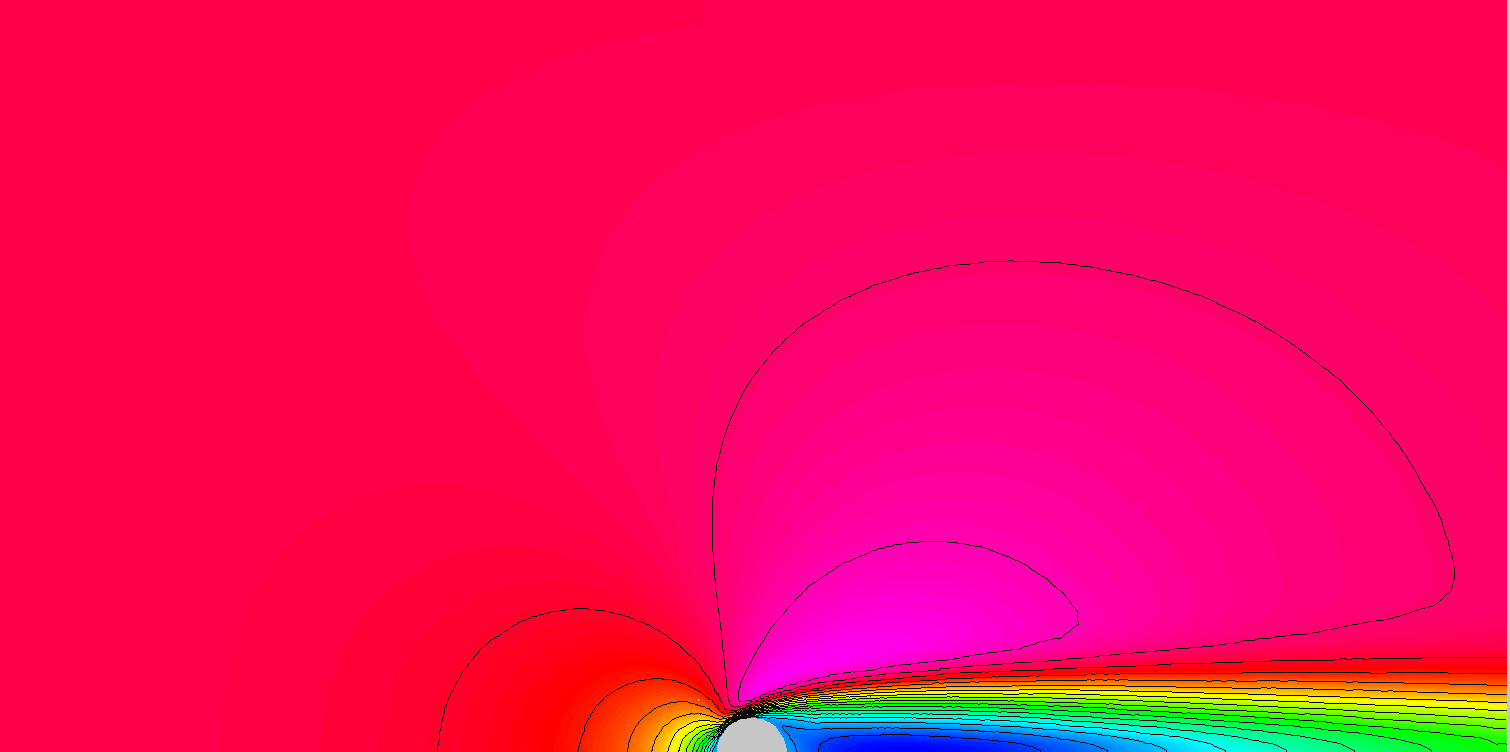
\includegraphics[width = \linewidth]{re80_vel_x} \\ (б)}
  \end{minipage}
\end{minipage}

\vspace{2mm}
\noindent
\begin{minipage}{\linewidth}
  \begin{minipage}{0.49\linewidth}
    \center{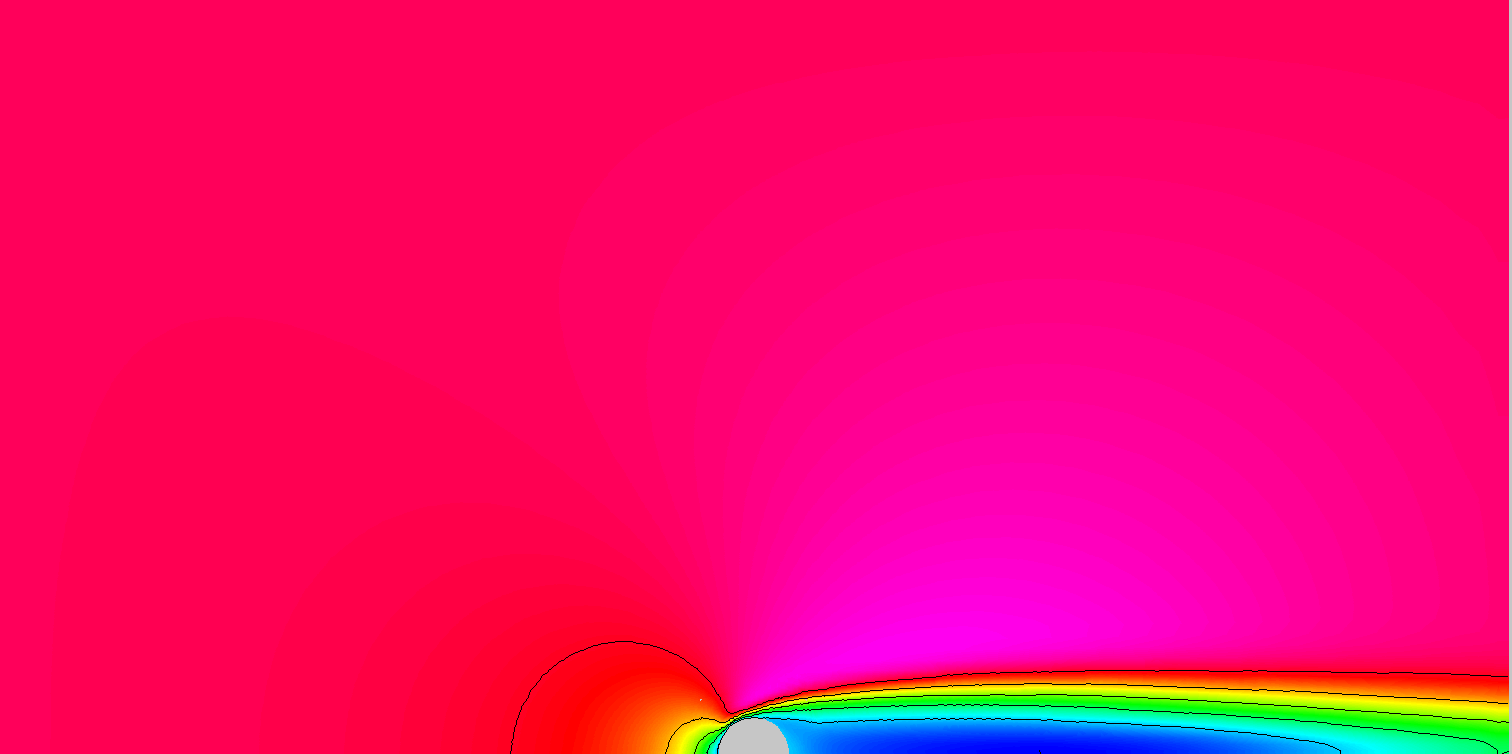
\includegraphics[width = \linewidth]{re130_vel_x} \\ (в)}
  \end{minipage}
  \hfill
  \begin{minipage}{0.49\linewidth}
    \center{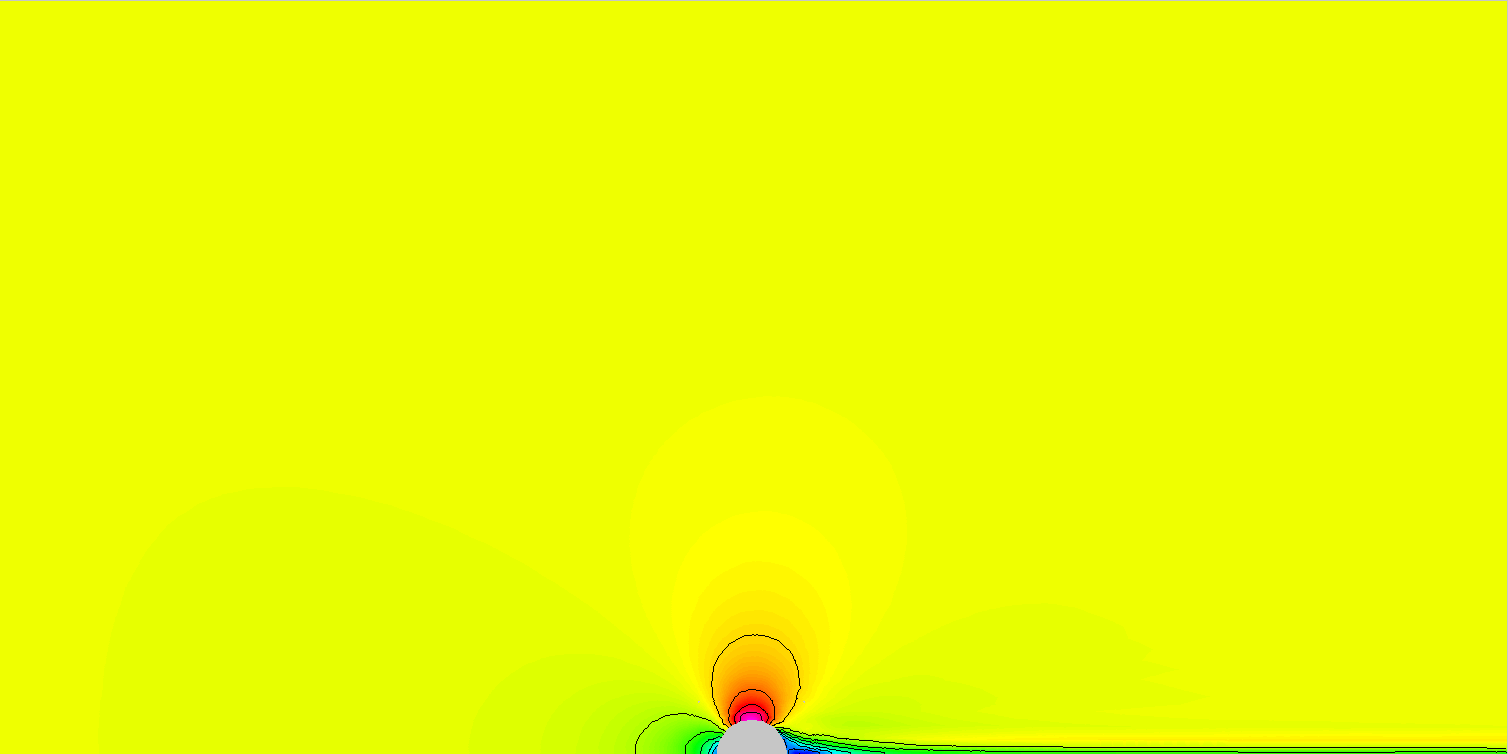
\includegraphics[width = \linewidth]{vel_x} \\ (г)}
  \end{minipage}
\end{minipage}
\piccapt{Распределение продольной компоненты скорости: (a) - $Re = 40$, (б) - $Re = 80$, \\(в) - $Re = 130$, (г) - невязкая жидкость.}

\noindent На рисунке 4 можно видеть, что внутри рециркуляционной зоны скорость близка к нулю, а на продольной границе рециркуляционной зоны скорость принимает максимальное значение. В случае с невязкой жидкостью (рис. 4(г)), скорость потока максимальна в области, находящейся над цилиндром.

\newpage
\subsection{Распределение поперечной компоненты скорости}

\begin{minipage}{\linewidth}
  \begin{minipage}{0.49\linewidth}
    \center{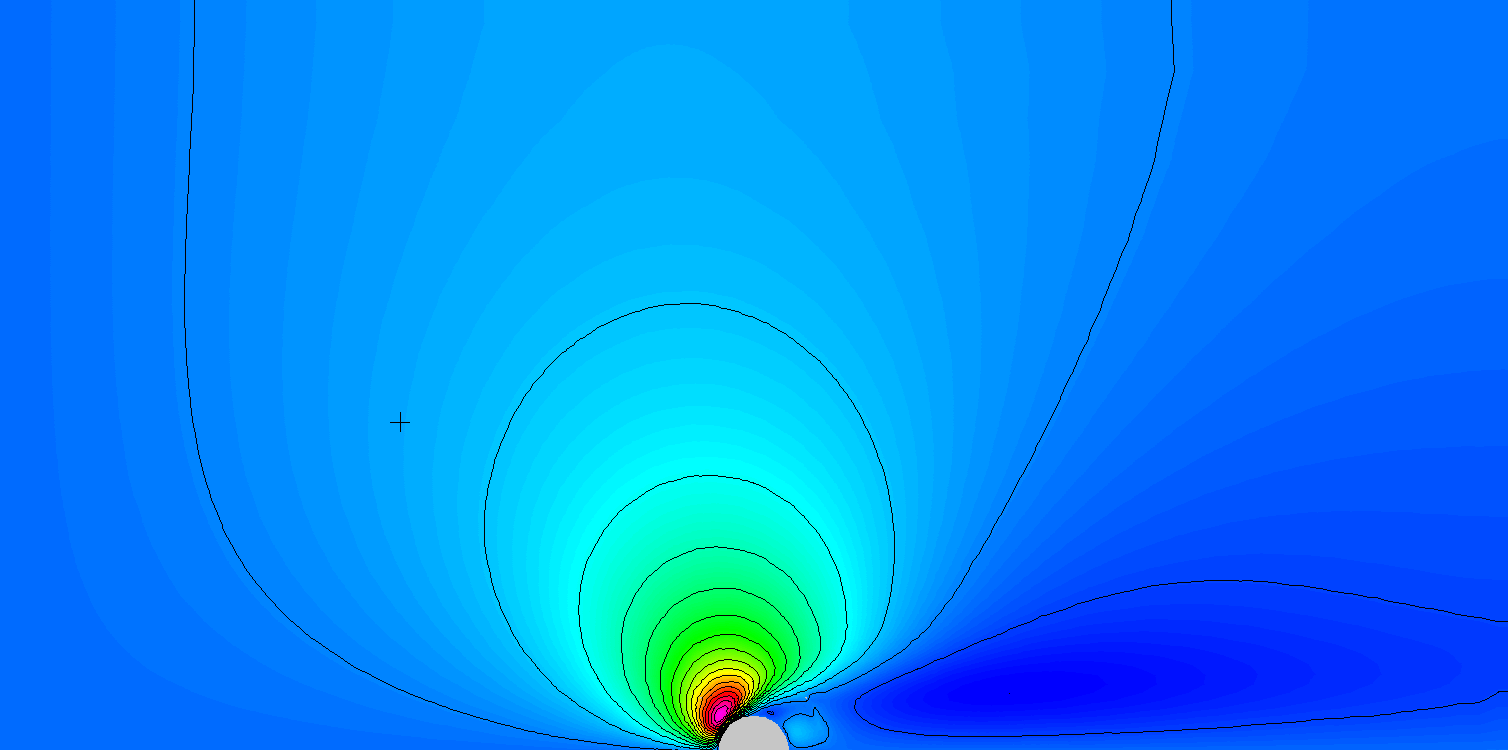
\includegraphics[width = \linewidth]{re_40_vel_y} \\ (a)}
  \end{minipage}
  \hfill
  \begin{minipage}{0.49\linewidth}
    \center{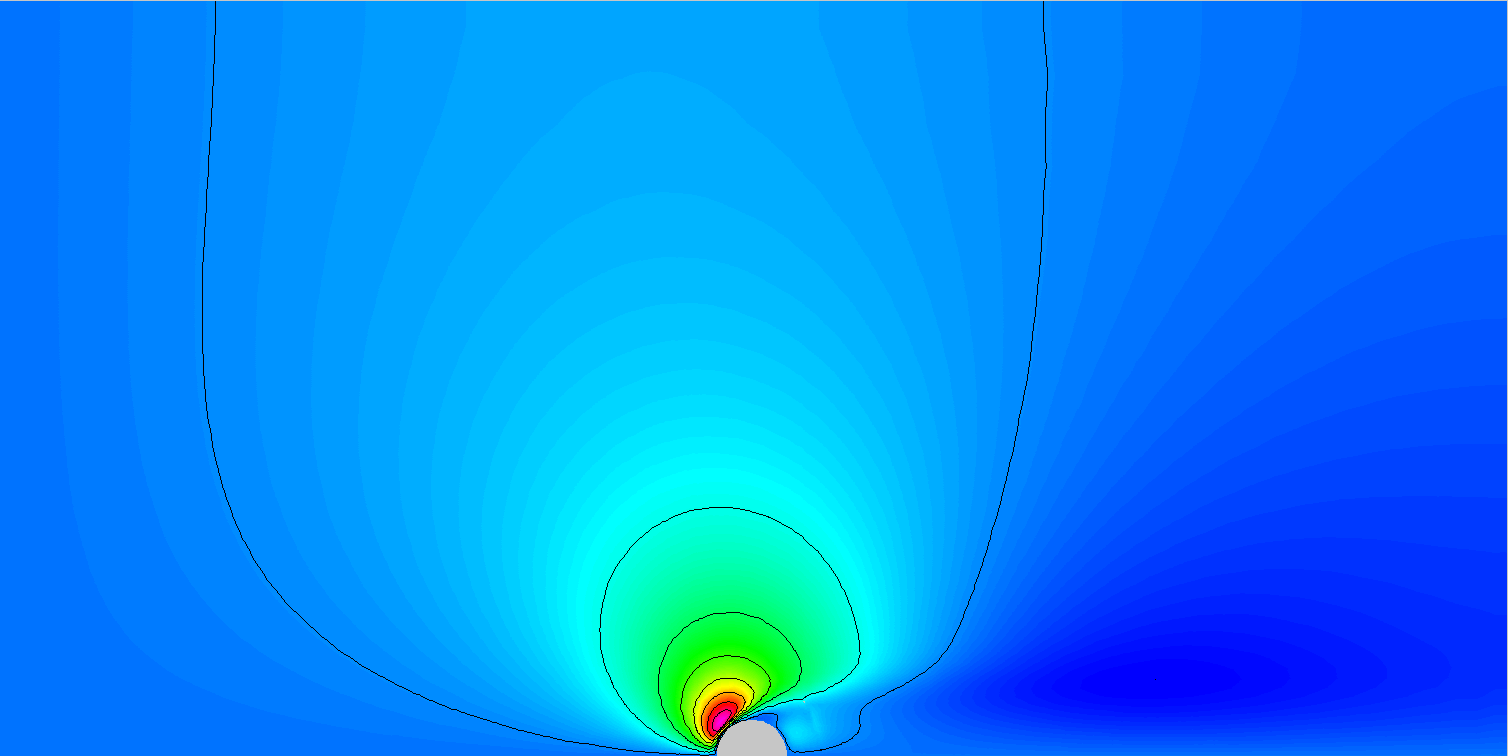
\includegraphics[width = \linewidth]{re80_vel_y} \\ (б)}
  \end{minipage}
\end{minipage}

\vspace{2mm}
\noindent
\begin{minipage}{\linewidth}
  \begin{minipage}{0.49\linewidth}
    \center{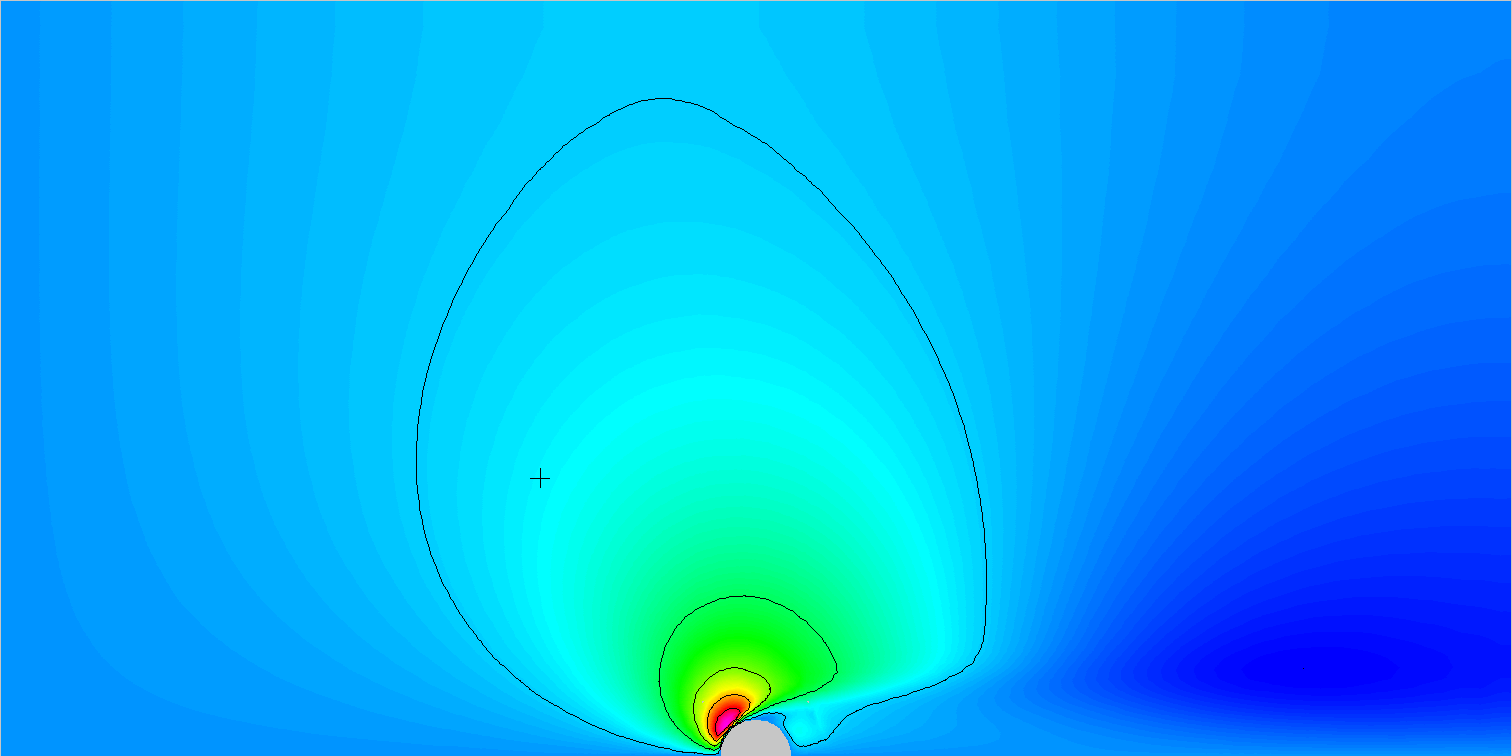
\includegraphics[width = \linewidth]{re130_vel_y} \\ (в)}
  \end{minipage}
  \hfill
  \begin{minipage}{0.49\linewidth}
    \center{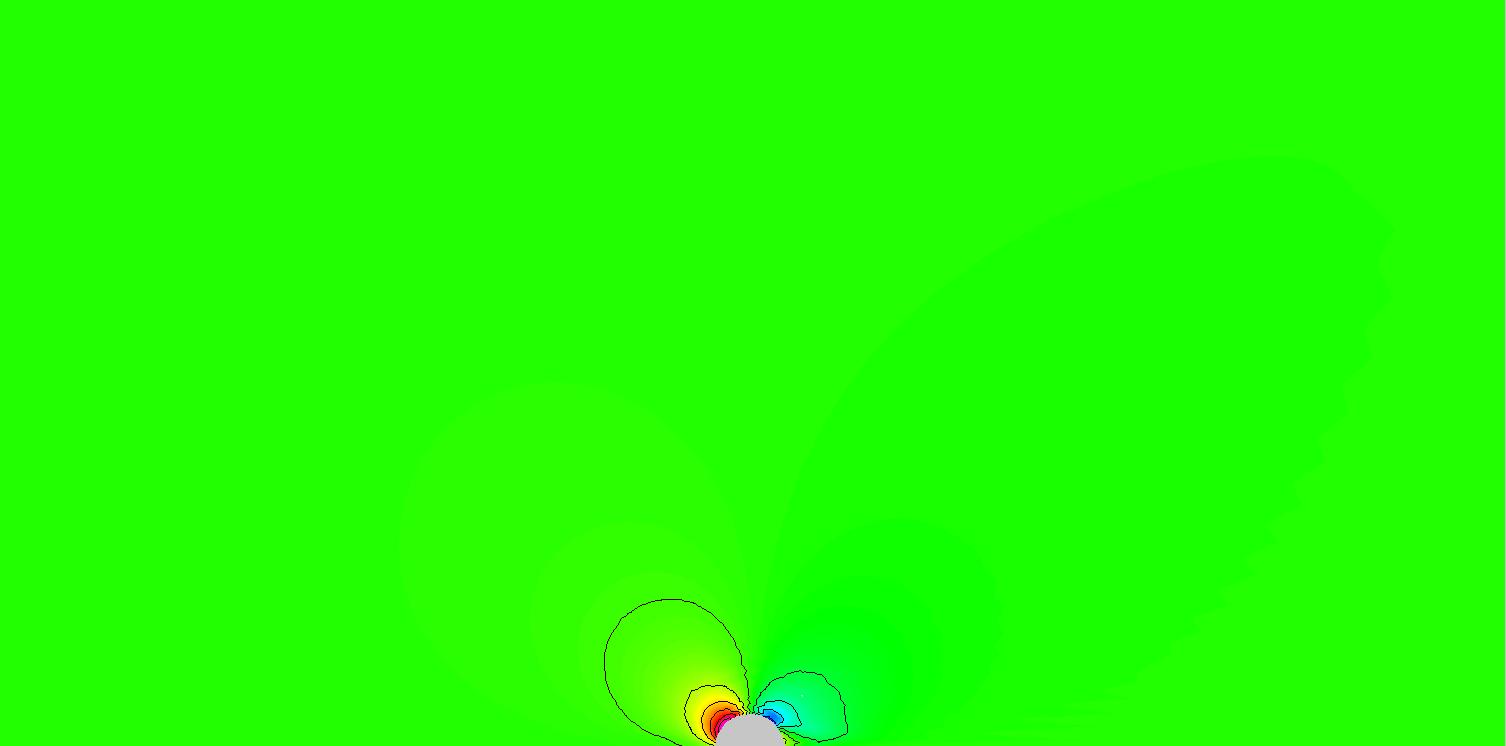
\includegraphics[width = \linewidth]{vel_y} \\ (г)}
  \end{minipage}
\end{minipage}
\piccapt{Распределение поперечной компоненты скорости: (a) - $Re = 40$, (б) - $Re = 80$, \\(в) - $Re = 130$, (г) - невязкая жидкость.}

\noindent Во всех случаях (рис. 5) можно видеть, что поперечная компонента скорости максимальна в области, находящейся слева от цилиндра, т.е. со стороны набегающего потока.

\newpage
\subsection{Распределение модуля скорости}

\begin{minipage}{\linewidth}
  \begin{minipage}{0.49\linewidth}
    \center{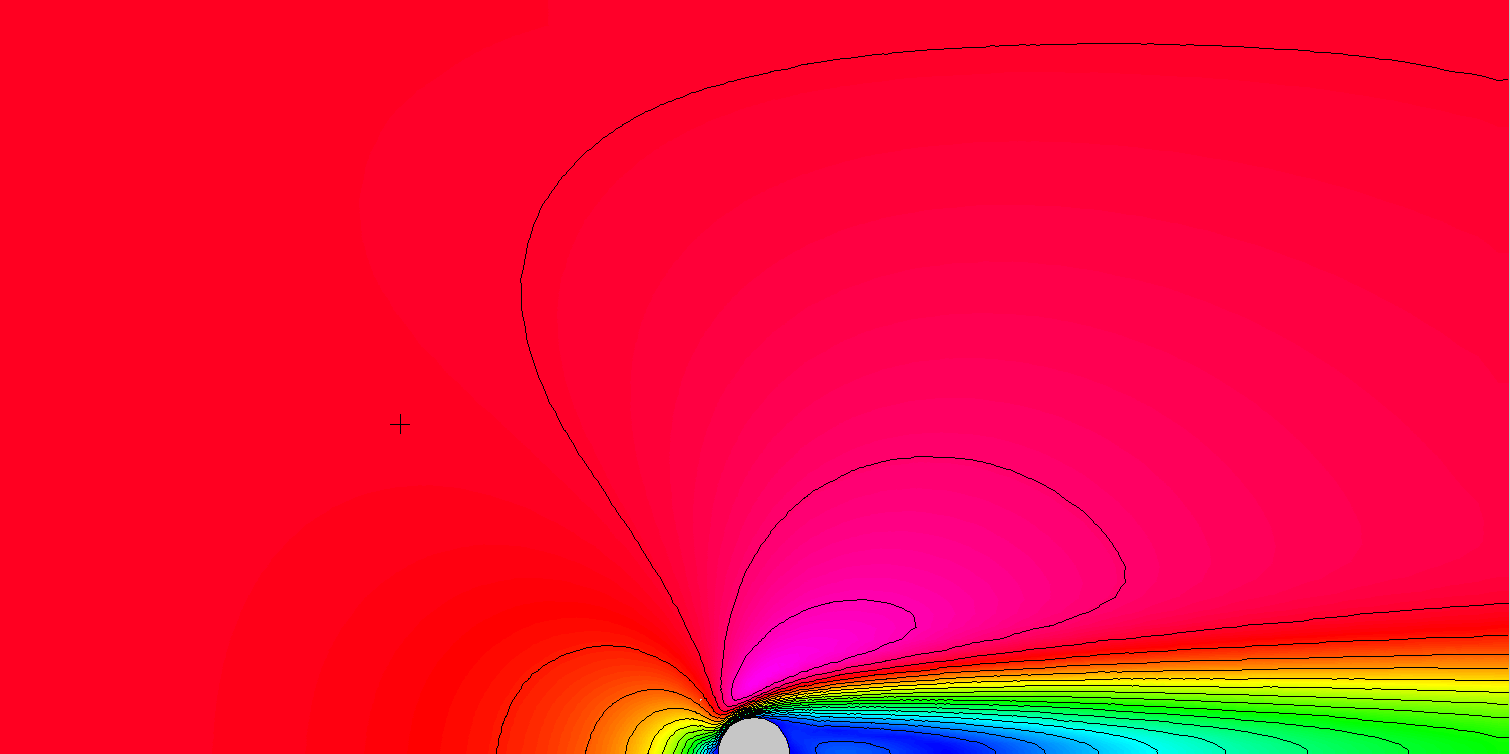
\includegraphics[width = \linewidth]{re_40_vel_wh} \\ (a)}
  \end{minipage}
  \hfill
  \begin{minipage}{0.49\linewidth}
    \center{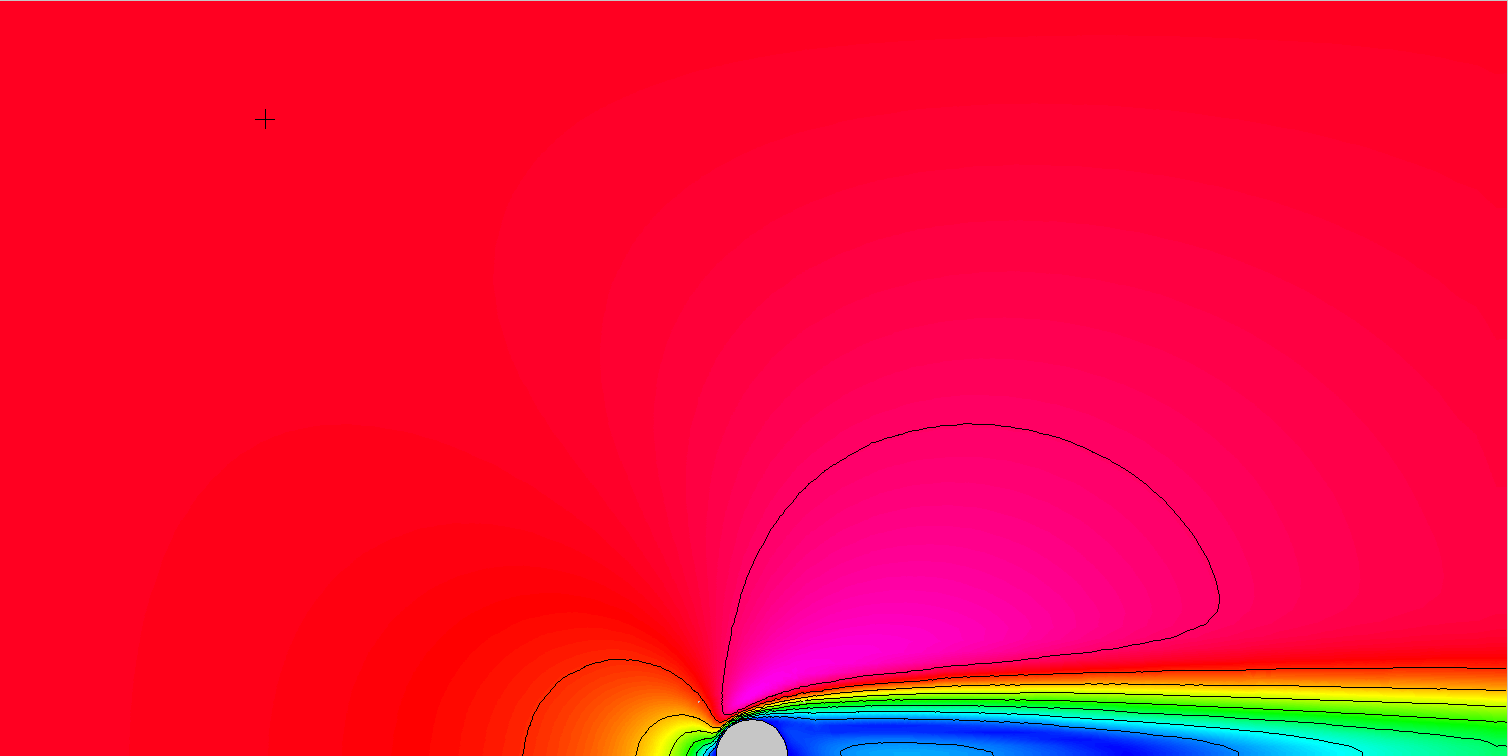
\includegraphics[width = \linewidth]{re80_vel_wh} \\ (б)}
  \end{minipage}
\end{minipage}

\vspace{2mm}
\noindent
\begin{minipage}{\linewidth}
  \begin{minipage}{0.49\linewidth}
    \center{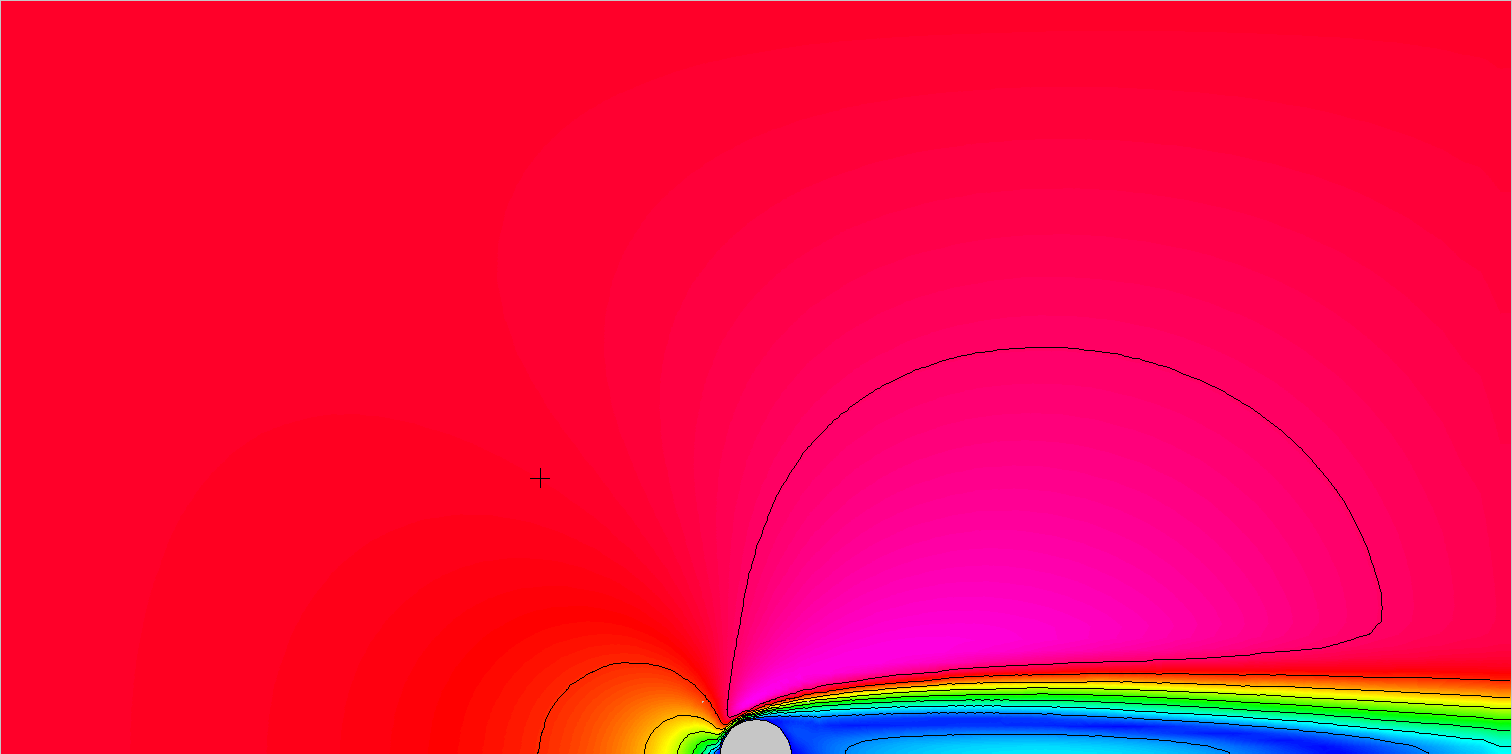
\includegraphics[width = \linewidth]{re130_vel_wh} \\ (в)}
  \end{minipage}
  \hfill
  \begin{minipage}{0.49\linewidth}
    \center{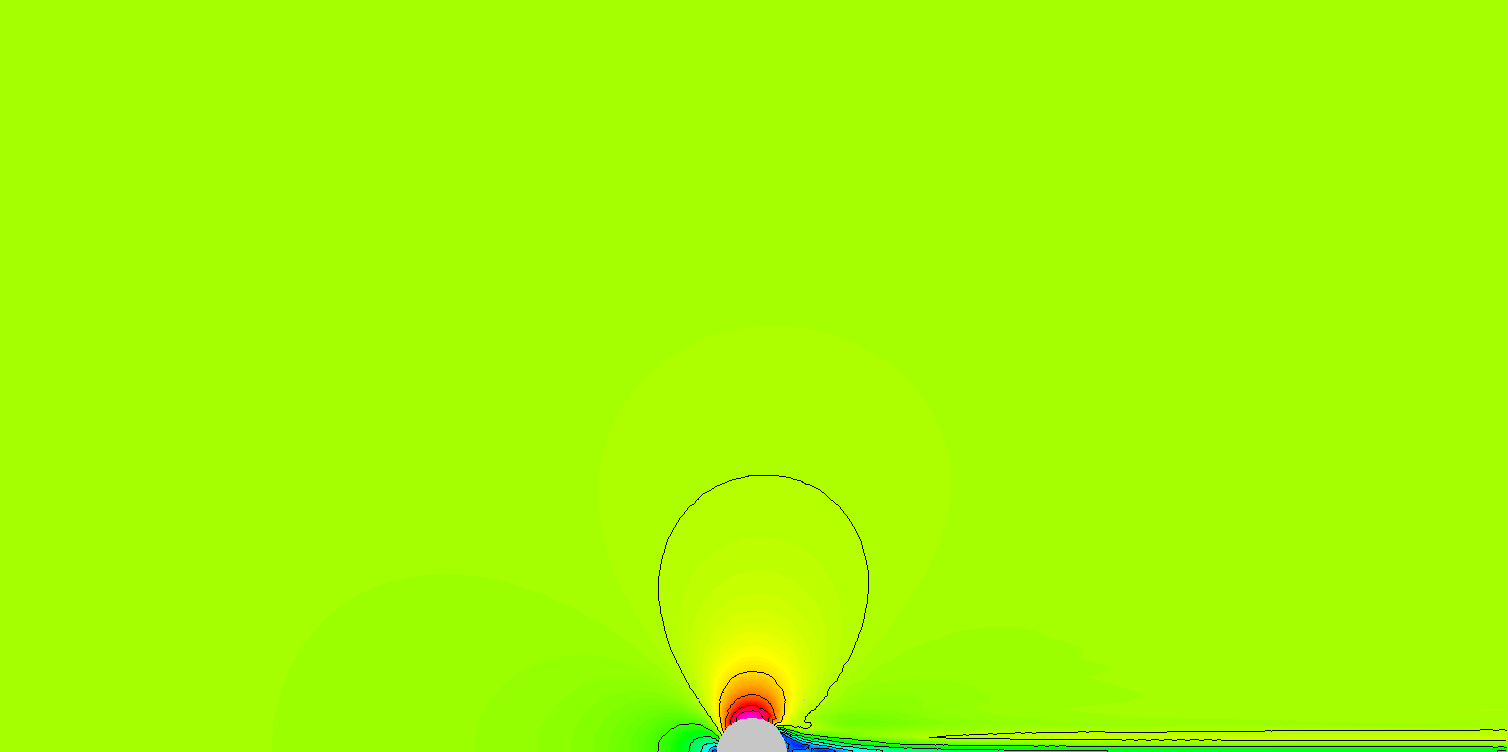
\includegraphics[width = \linewidth]{vel_wh} \\ (г)}
  \end{minipage}
\end{minipage}
\piccapt{Распределение модуля скорости: (a) - $Re = 40$, (б) - $Re = 80$, \\(в) - $Re = 130$, (г) - невязкая жидкость.}

\noindent Поскольку вклад поперечной компоненты скорости (рис.4) мал, по сравнению с продольной (рис.5), то картина распределения модуля скорости (рис. 6) очень близка к распредлению ее продольной компоненты.

\newpage
\subsection{Распределение давления}

\begin{minipage}{\linewidth}
  \begin{minipage}{0.49\linewidth}
    \center{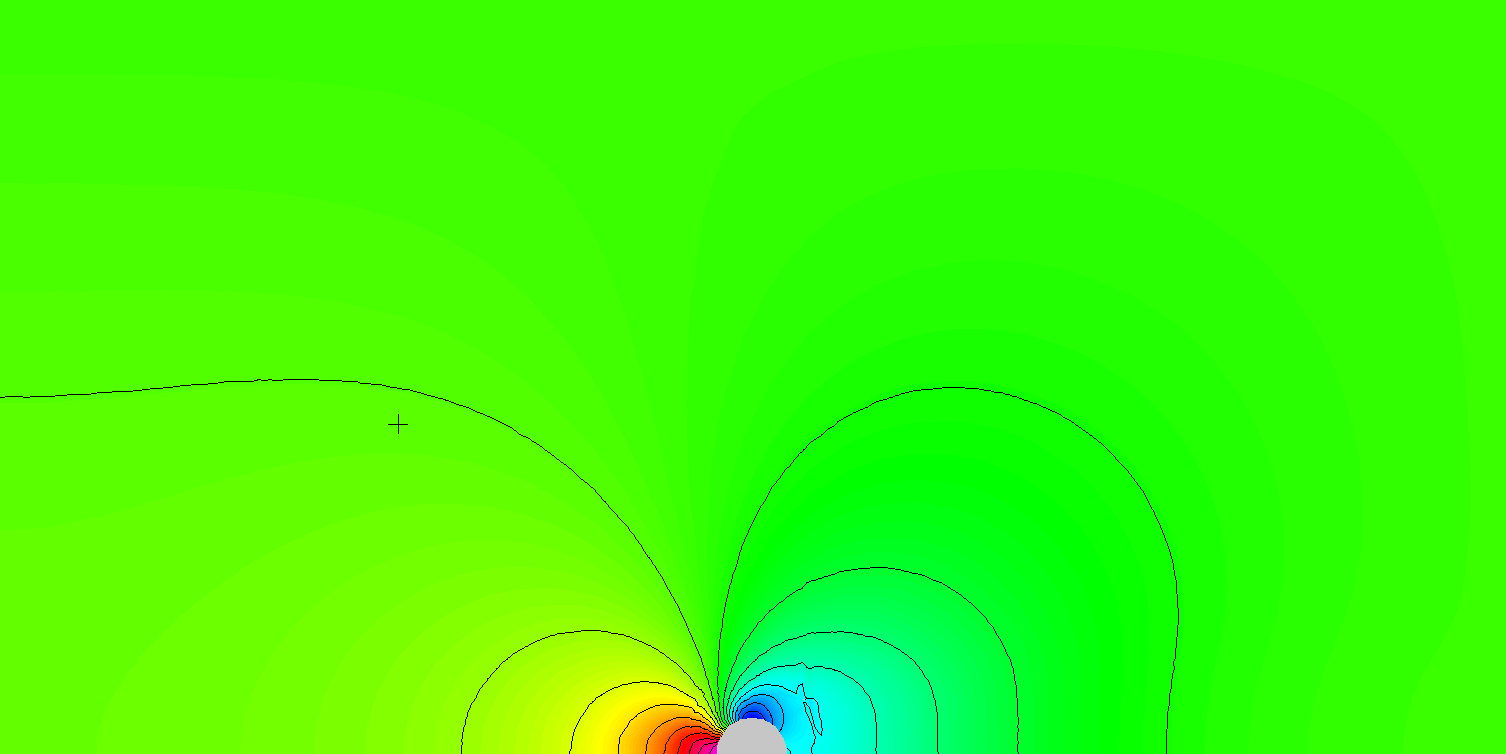
\includegraphics[width = \linewidth]{re_40_press} \\ (a)}
  \end{minipage}
  \hfill
  \begin{minipage}{0.49\linewidth}
    \center{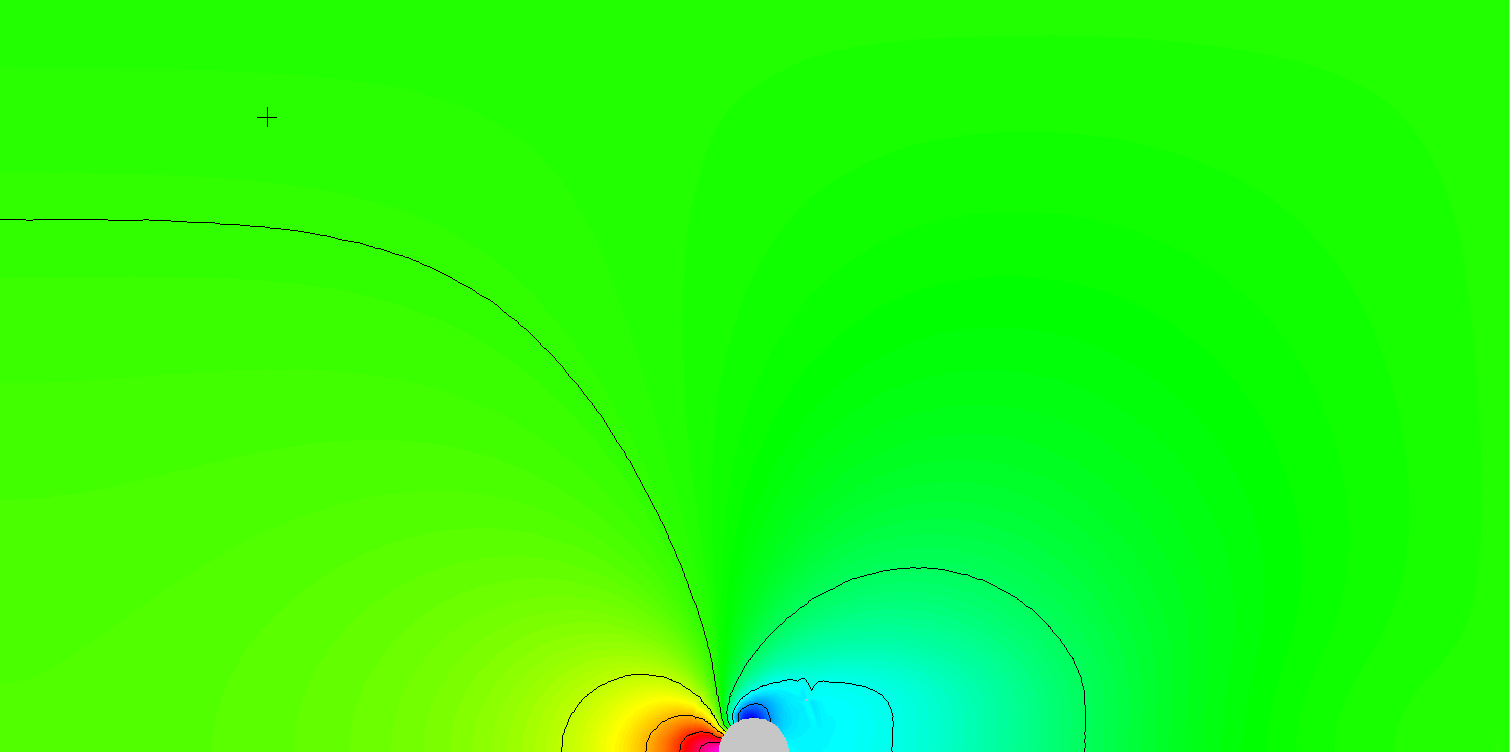
\includegraphics[width = \linewidth]{re_80_press} \\ (б)}
  \end{minipage}
\end{minipage}

\vspace{2mm}
\noindent
\begin{minipage}{\linewidth}
  \begin{minipage}{0.49\linewidth}
    \center{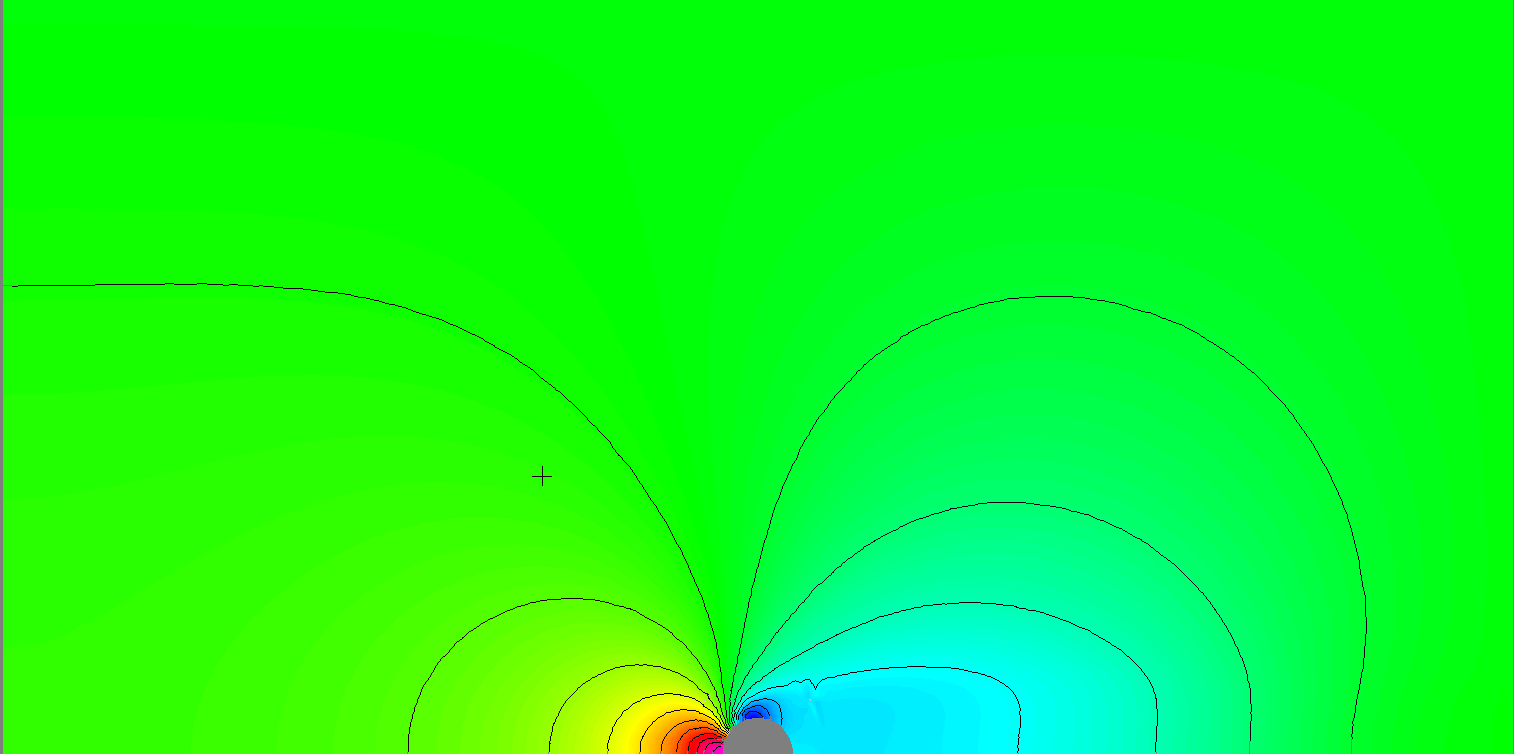
\includegraphics[width = \linewidth]{re130_press} \\ (в)}
  \end{minipage}
  \hfill
  \begin{minipage}{0.49\linewidth}
    \center{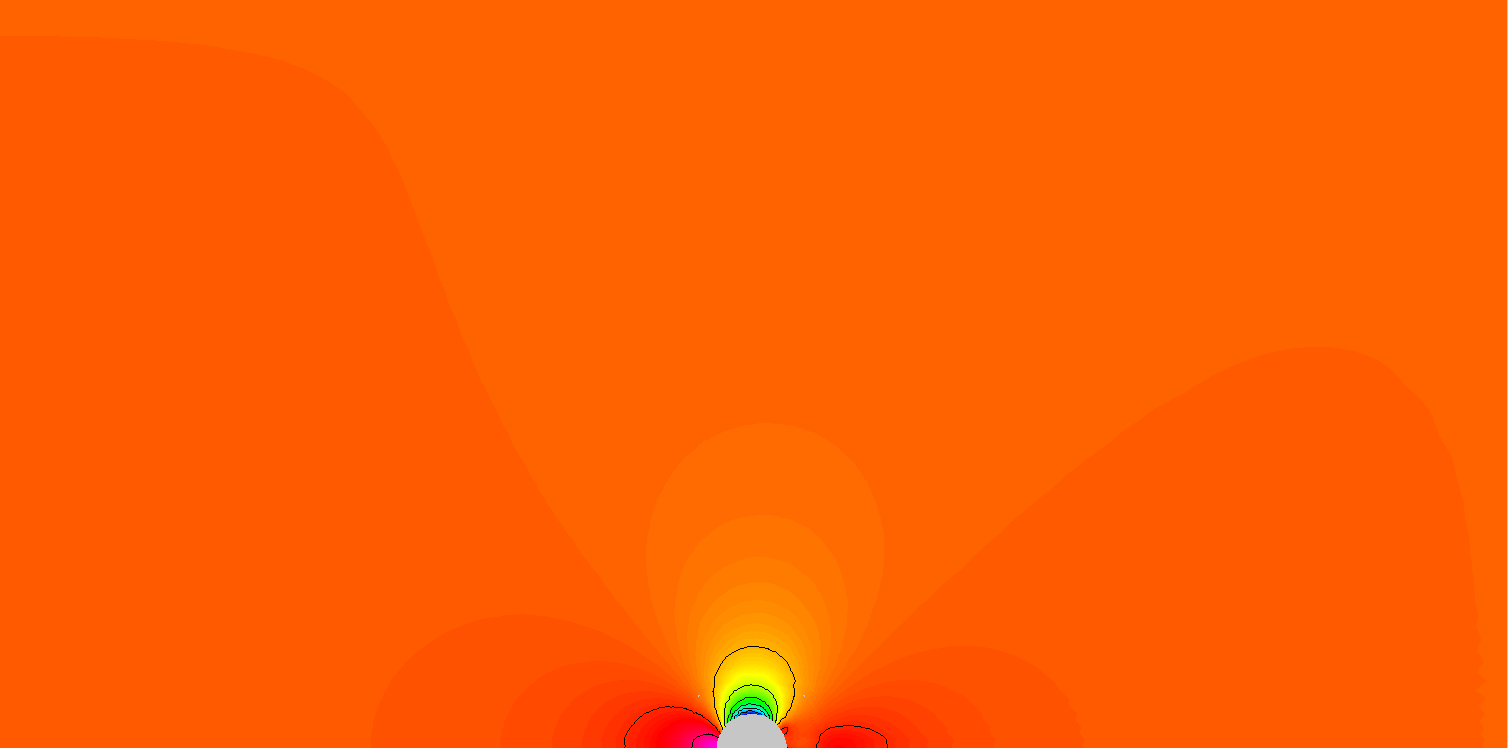
\includegraphics[width = \linewidth]{press} \\ (г)}
  \end{minipage}
\end{minipage}
\piccapt{Распределение давления: (a) - $Re = 40$, (б) - $Re = 80$, \\(в) - $Re = 130$, (г) - невязкая жидкость.}

\noindent В случае вязкой жидкости (рис. 7(а, б, в)) зона максимального давления находится слева от цилиндра (со стороны набегающего потока). По другую сторону цилиндра, наблюдается зона пониженного давления, и она тем больше, чем больше $Re$. В случае невязкой жидкости (рис. 7(г)) картина распределения давления примерно симметрична.

\subsection{Максимальные значения давления и скорости}

\begin{center}
  {\small\tabcapt{Макс. значения скорости и давления.}}
  \begin{tabular}[h!]{p{4cm}|>{\centering}p{2cm}|>{\centering}p{2cm}}
  \bf Тип жидкости & $V_{max}$ & $p_{max}$\ntb
  \hline  
  \hline  
   Вязкая, $Re = 40$  & 1.173 & 0.569  \ntb
   Вязкая, $Re = 80$  & 1.182 & 0.545 \ntb
   Вязкая, $Re = 130$ & 1.187 & 0.539 \ntb
  \hline  
  Невязкая & 1.86 & 0.505 \ntb
  \end{tabular}
\end{center}

В случае вязкой жидкости с увеличением $Re$ наблюдается увеличение максимальной скорости и уменьшение максимального давления. В случае невязкой жидкости максимальная скорость в потоке существенно больше, чем в случае с вязкой жидкостью, а максимальное давление меньше. 

\subsection{Распределение коэффициента давления $C_p$}

\pic{1}{cp}{\small Зависимость коэффициента давления от полярного угла \\ между радиусом окружности цилиндра и осью $Ox$. }

На рисунке 8 можнов видеть, что аналитические и расчетные значения близки лишь при маленьких полярных углах. При увеличении полярного угла, для вязкой жидкости, расчетный $C_{p_{\text{расч.}}}$ существенно отличается, от $C_{p_{\text{ан.}}} = 1 - 4\sin^2{\varepsilon}$ ($\varepsilon$ - полярный угол) для идеальной жидкости, в то время как для невязкой жидкости, графики расчетного и аналитического коэффициентов давления намного ближе (что просто подтверждает теорию для невязкой жидкости).

\n
При малых углах, в случае вязкой жидкости, значение коэффициента давления при малых значения $Re$ больше, но при увеличении угла ситуация меняется на обратную. 

\newpage
\subsection{Длина рециркуляционной зоны}

$L_{\text{р.}}$ -- длина рециркуляционной зоны, полученная при расчетах.

\n\noindent
\begin{minipage}{\linewidth}
  \begin{minipage}{0.49\linewidth}
    \begin{center}
       {\small\tabcapt{Зависимость $L_{\text{р.}}$ от $Re$.}}
      \begin{tabular}[h!]{p{3cm}|>{\centering}p{3cm}}
        \bf $Re$ & $L_{\text{р.}}$  \ntb
        \hline  
        \hline  
        $Re = 40$  & 2.68\ntb
        $Re = 80$  & 5.24\ntb
        $Re = 130$ & 8.07\ntb
      \end{tabular}
    \end{center}
  \end{minipage}
  \hfill
  \begin{minipage}[t]{0.49\linewidth}
    Длина рециркуляционной зоны увеличивается вместе с числом Рейнольдса $Re$. Зависимость $L_{\text{р.}}$ от $Re$ линейная. 
  \end{minipage}
\end{minipage}

\n
\subsection{Коэффициент сопротивления цилиндра $C_D$}

$D_{\text{расч.}}$ -- полное сопротивления цилиндра в потоке, полученное при расчетах программным пакетом FLOS.\\
$C_{D_{\text{ан.}}}$ -- коэффициент сопротивления цилиндра, полученный при помощи формулы:

\begin{equation*}
C_{D_{\text{ан.}}} = 4D_{\text{ан.}}, \quad D_{\text{ан.}} = \int\limits_{AB}(p + \rho V_{x}^{2})ds - \int\limits_{EF}(p + \rho V_{x}^{2})ds - \int\limits_{BE}(p + \rho V_x V_y)ds 
\end{equation*}

\n
\noindent $C_{D_{\text{эксп.}}}$ -- коэффициент сопротивления цилиндра, полученный экспериментально:

\n
\pic{0.8}{teor}{Зависимость коэффициента сопротивления круглых цилиндров от числа $Re$.}

\newpage
\begin{center}
  {\small\tabcapt{Сравнение расчетного, аналитического и \\ экспериментального коэффициента $C_d$}}
  \begin{tabular}[h!]{p{4cm}|>{\raggedleft}p{2cm}>{\raggedleft}p{2cm}|>{\raggedleft}p{2cm}>{\raggedleft}p{2cm}}
  \bf Тип жидкости & $D_{\text{ан.}}$ & $D_{\text{расч.}}$ & $C_{D_{\text{ан.}}}$ & $C_{D_{\text{эксп.}}}$ \ntb
  \hline  
  \hline  
   Вязкая, $Re = 40$  & 0.3686 & 0.3867 & 1.4744 & $\approx 1.75$  \ntb
   Вязкая, $Re = 80$  & 0.2995 & 0.3010 & 1.1980 & $\approx 1.50$ \ntb
   Вязкая, $Re = 130$ & 0.2594 & 0.2578 & 1.0376 & $\approx 1.30$ \ntb
  \hline  
  Невязкая & 0.0161 & 0.0149 & 0.0644 & -------- \ntb
  \end{tabular}
\end{center}

Видно, что рассчетные и аналитические данные для вязкой жидкости совпадают, однако, значения экспериментальных данных несколько выше. Для невязкой жидкости полученные коэффициенты сопротивления на порядок меньше, и можно говорить о их приближенном равенстве нулю по сравнению с вязкой жидкостью, что согласуется с теорией.
 
\section{Вывод}
В ходе работы было проанализированно обтекание круглого цилиндра вязкой и невязкой жидкостью, влияние числа Рейнольдса на поле скорости и давления (п. 3.1 - 3.5), на длину рецикуляционной зоны (п. 3.8). Так же были произведены сравнения аналитических и расчетных данных для коэффициента споротивления цилиндра (п. 3.9) и коэффициента давления (п. 3.7) по контуру цилиндра. В целом, расчетные значения во всех опытах были близки к аналитическим и экспериментальным.

\end{document}	
	